%%
% TUM Corporate Design LaTeX Templates
% Based on the templates from https://www.tum.de/cd
%
% Feel free to join development on
% https://gitlab.lrz.de/tum-templates/templates
% and/or to create an issue in case of trouble.
%
% tum-presentation class for scientific talks, thesis presentations, ...
%
%%

%\documentclass[4to3]{tum-presentation}
%\documentclass[navsym]{tum-presentation}
%\documentclass[nothreeliner]{tum-presentation}
%\documentclass[handout,4on1]{tum-presentation}
%\documentclass[handout,2on1]{tum-presentation}
%\documentclass[handout]{tum-presentation}
\documentclass{tum-presentation}

\addbibresource{literature.bib}

\title[Research Internship]{Research Internship with RCS@TUM}
\subtitle{Implementation of tiny machine learning models on microcontrollers}
\author[Philipp v. K.]{\textbf{Philipp van Kempen}}
\institute[]{Department of Electrical and Computer Engineering,
  Technical University of Munich (TUM)}
\date{\textbf{24.08.2020 - 25.10.2020}}

\footline{\insertshortauthor~|~\insertshorttitle}

\usepackage{multirow}
%\usepackage[table]{xcolor}
\usepackage[utf8]{inputenc}
\usepackage{multirow}
\usepackage{hhline}
\usepackage{colortbl}
\usepackage{multicol}
\usepackage{caption}
\usepackage{subcaption}
\usepackage{hyperref}

\begin{document}

\begin{frame}[noframenumbering]
  \titlepage
\end{frame}

\begin{frame}
  \frametitle{Motivation}
    \begin{multicols}{2}
  \begin{itemize}
      \item Machine learning in the past vs. today
      \item Compute-intensive algorithms
      \item State of the Art: ML/AI on smartphones
      \item Research topic: ML/AI on microcontrollers
  \end{itemize}

  \begin{figure}[h]
\centering
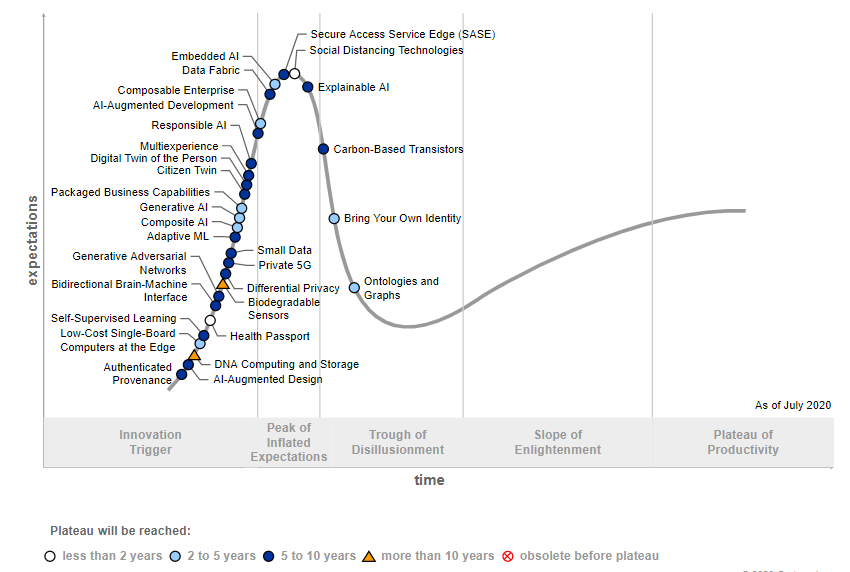
\includegraphics[width=0.45\textwidth]{figures/2020_08_23_medialist_gartner_hype_cycle_2020.png}
\caption{2020 Gartner Hype Cycle\footnote{\url{https://www.gartner.com/smarterwithgartner/5-trends-drive-the-gartner-hype-cycle-for-emerging-technologies-2020/}}}
\label{fig:gartner2020}
\end{figure}

  \end{multicols}
\end{frame}

\begin{frame}

\centering{
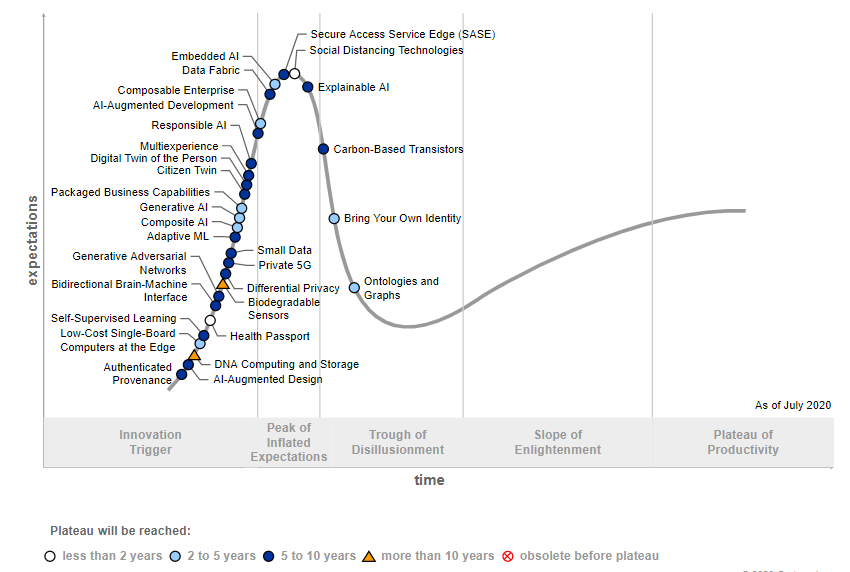
\includegraphics[width=0.7\textwidth]{figures/2020_08_23_medialist_gartner_hype_cycle_2020.png}}

\end{frame}

\begin{frame}
  \frametitle{Goals}
  
  \begin{itemize}
      \item 9 weeks
      \item Support Electronic System Level (ESL) research group (EDA+RCS)
      \item Implement reference implementations of TinyML models on STM32 Hardware
      \item Work based on previous attempts by Alex Hoffman
      \item Extend toolchain with new features and documentation
      \item Summarize results at the end of the internship
  \end{itemize}

\end{frame}

\begin{frame}
  \frametitle{Steps}
%\vspace{-5em}
  \begin{multicols}{2}
\textbf{Major topics:}

\begin{itemize}
    \item Reading books and web pages
    \item Toolchain setup and extension
    \item Training of examples
    \item Implementation of examples
    \item Documentation and handover
\end{itemize}
  \begin{figure}[h]
\centering
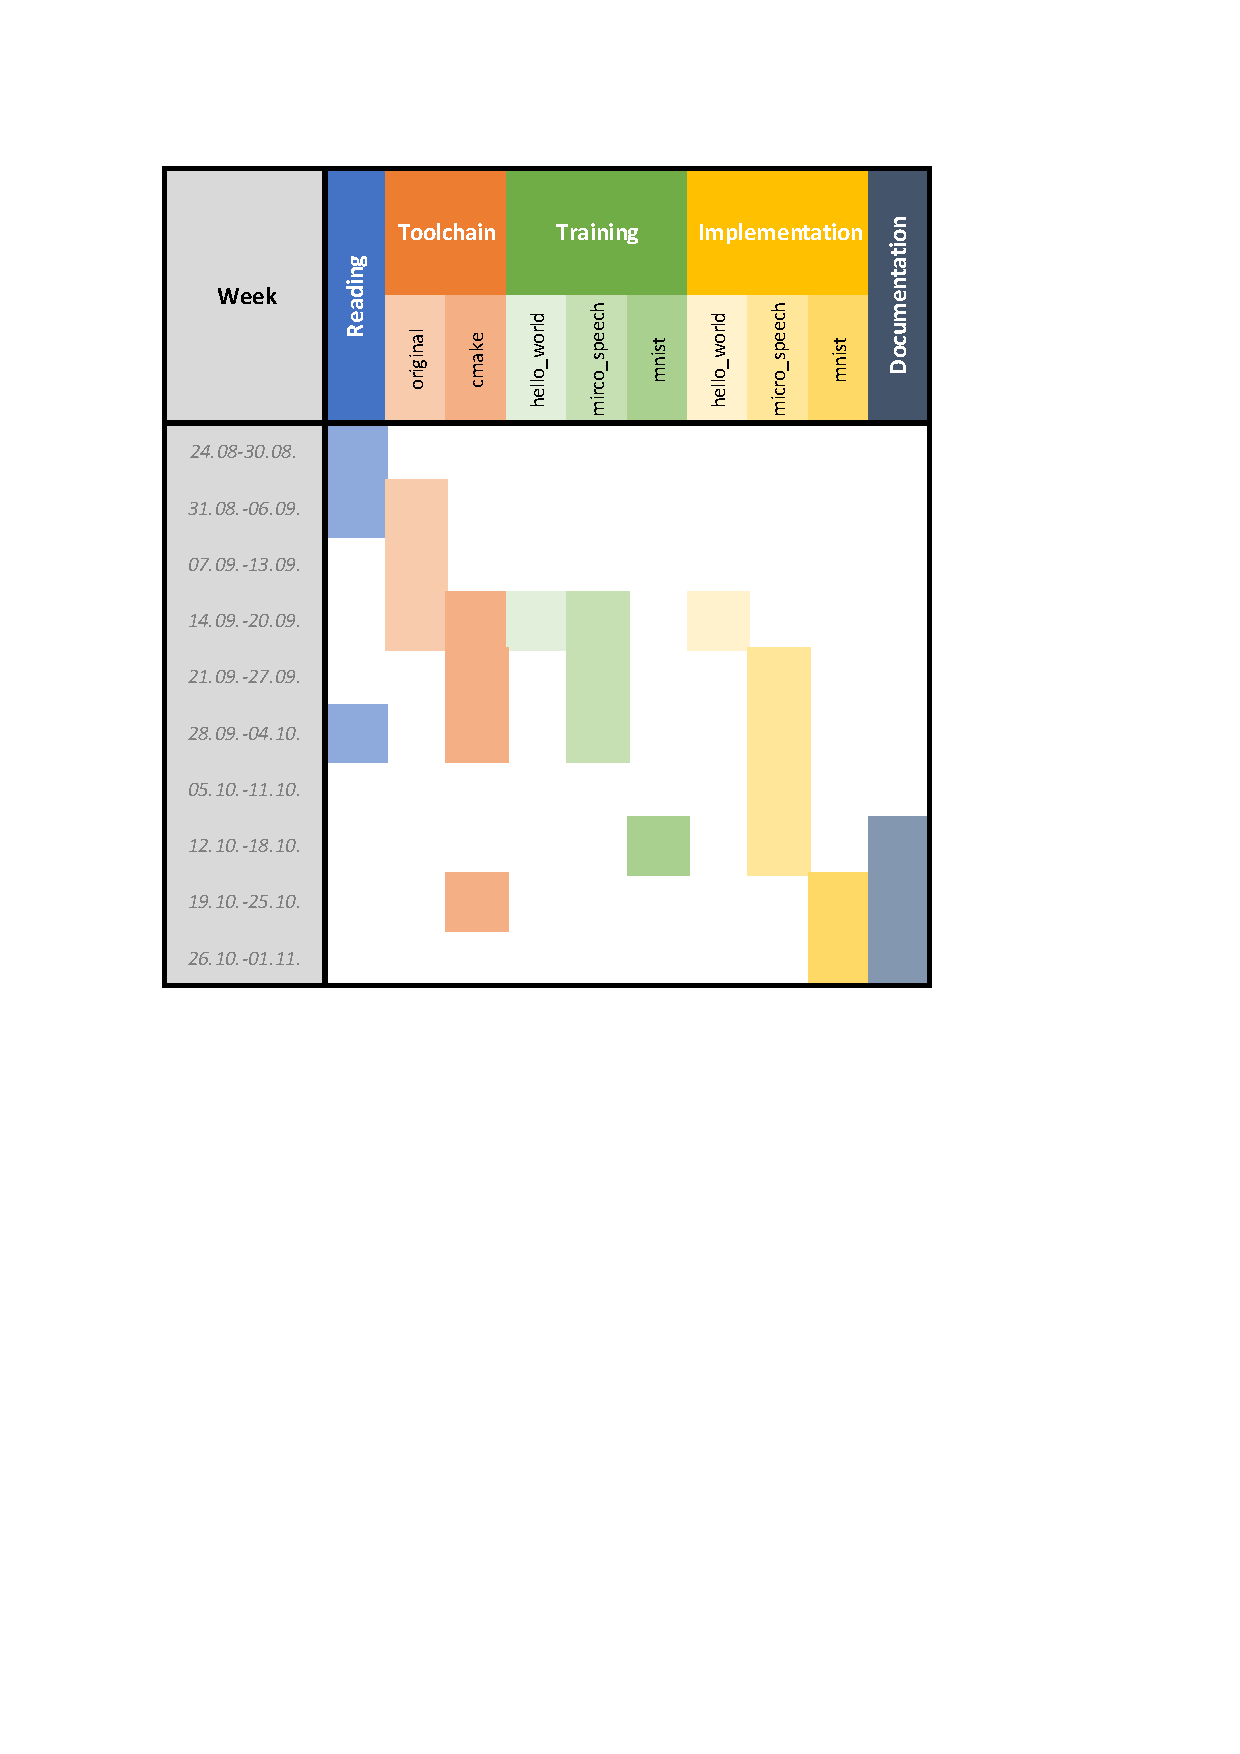
\includegraphics[scale=0.6]{figures/fp_report_plan.pdf}
\caption{Schedule}
\label{fig:schedule}
\end{figure}
  \end{multicols}

\end{frame}

\begin{frame}
  \frametitle{Reading}
  
  \begin{multicols}{2}

\begin{itemize}
    \item Book by Pete Warden and Daniel Situnayake
    \item Introduction to Tensorflow Lite for Microcontrollers (TFLM) framework
    \item Referencing examples located in the Tensorflow source tree
    \begin{itemize}
        \item \textbf{Hello World}
        \item \textbf{Micro Speech}
    \end{itemize}
    \item Official documentation of Tensorflow (v1.5 and latest)
\end{itemize}

    \begin{figure}[h]
\centering
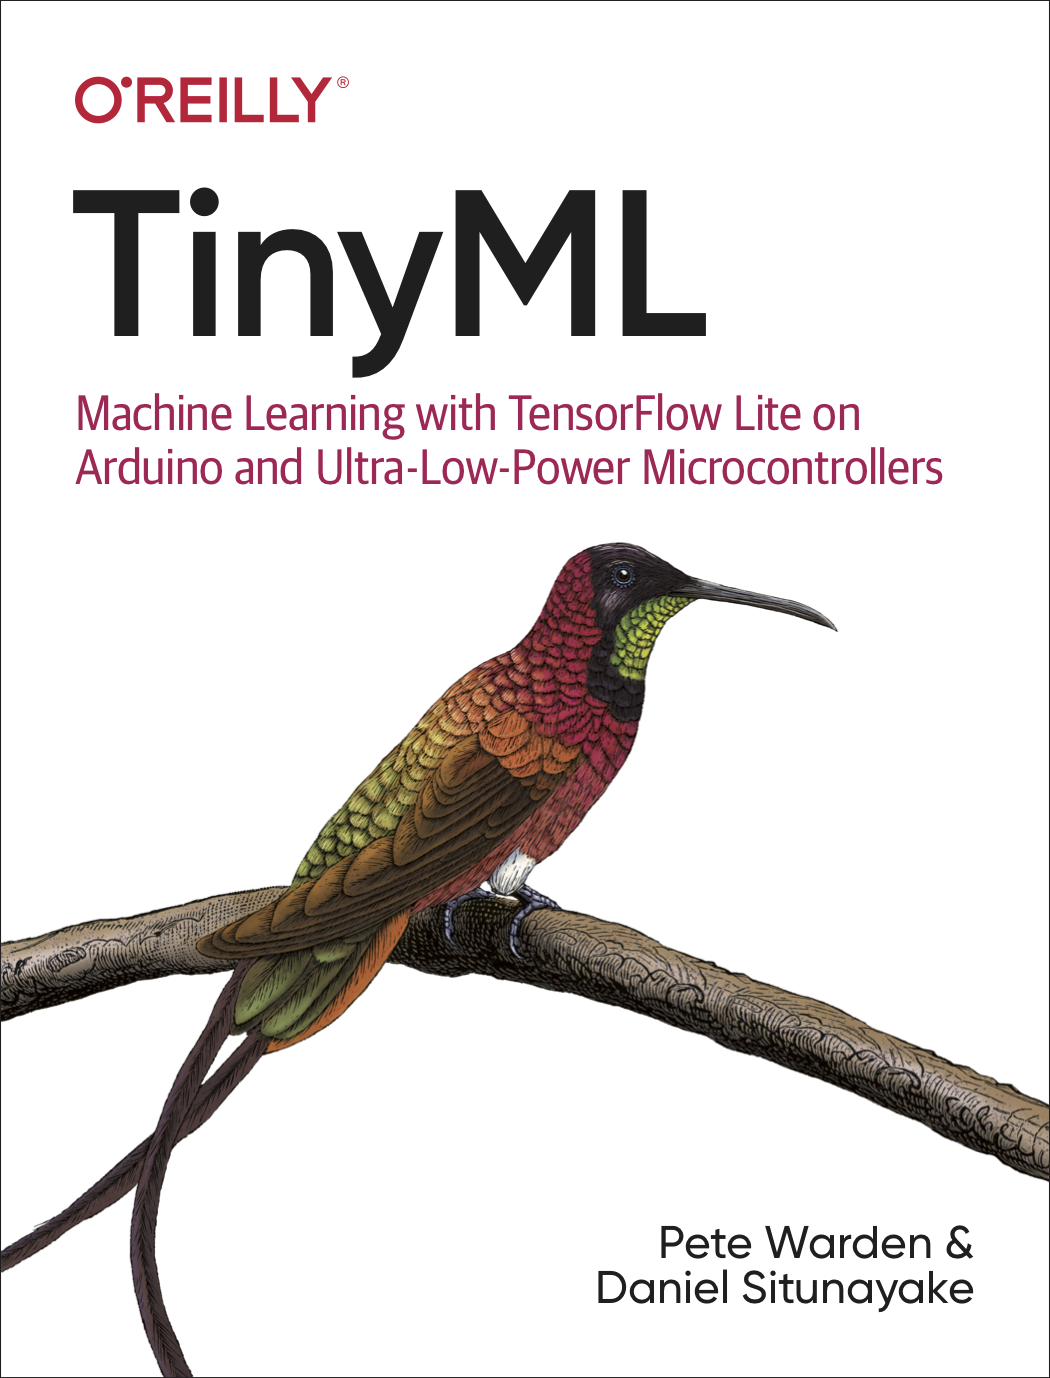
\includegraphics[width=.2\textwidth]{figures/tinyml_cover2.png}
\caption{TinyML Book\footnote{\url{https://tinymlbook.com}}}
\label{fig:schedule}
\end{figure}

\end{multicols}

\end{frame}

\begin{frame}
  \frametitle{Toolchain}

\begin{itemize}
    \item Original ARM mBed toolchain used as a reference
    \item CMake based - Initially developed by Konstantin Oblaukhov \footnote{\url{https://github.com/ObKo/stm32-cmake}}, Improved and extended by Alex Hoffman
    \item Reference Application: \lstinline{STM3240G-EVAL-TensorFlow-MNIST}
    \item Some workarounds required to fix upstream bugs
\end{itemize}

\begin{figure}[h]
     \centering
     \begin{subfigure}[b]{0.49\textwidth}
         \centering
         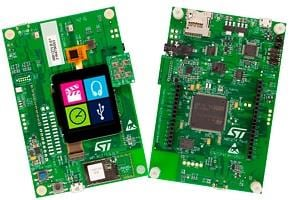
\includegraphics[width=0.45\textwidth]{figures/disco_f413h.jpg}
         \caption{STM32F413H-DISCOVERY}
         \label{fig:stm32f4}
     \end{subfigure}
     \hfill
     \begin{subfigure}[b]{0.49\textwidth}
         \centering
         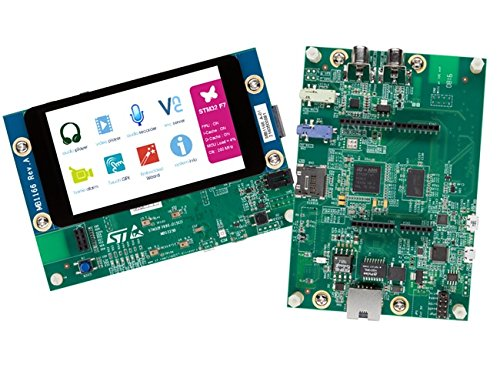
\includegraphics[width=0.45\textwidth]{figures/disco_f769i.jpg}
         \caption{STM32F769I-DISCOVERY}
         \label{fig:stm32f7}
     \end{subfigure}
        \caption{Target Boards\footnote{Images taken from \url{https://www.st.com}}}
        \label{fig:boards}
\end{figure}

\end{frame}

\begin{frame}
  \frametitle{Training}
  
  \begin{itemize}
      \item Training scripts: Interactive notebooks hosted on Google Colaboratory\footnote{\url{https://colab.research.google.com}}
      \item Deployment on Microcontrollers:
      \begin{itemize}
          \item Quantization
          \item Optimizations
          \item Conversion to TFLite
          \item Interpreter vs. Compiled offline model
      \end{itemize}
  \end{itemize}
  \vspace{-5em}
  \hspace{20em}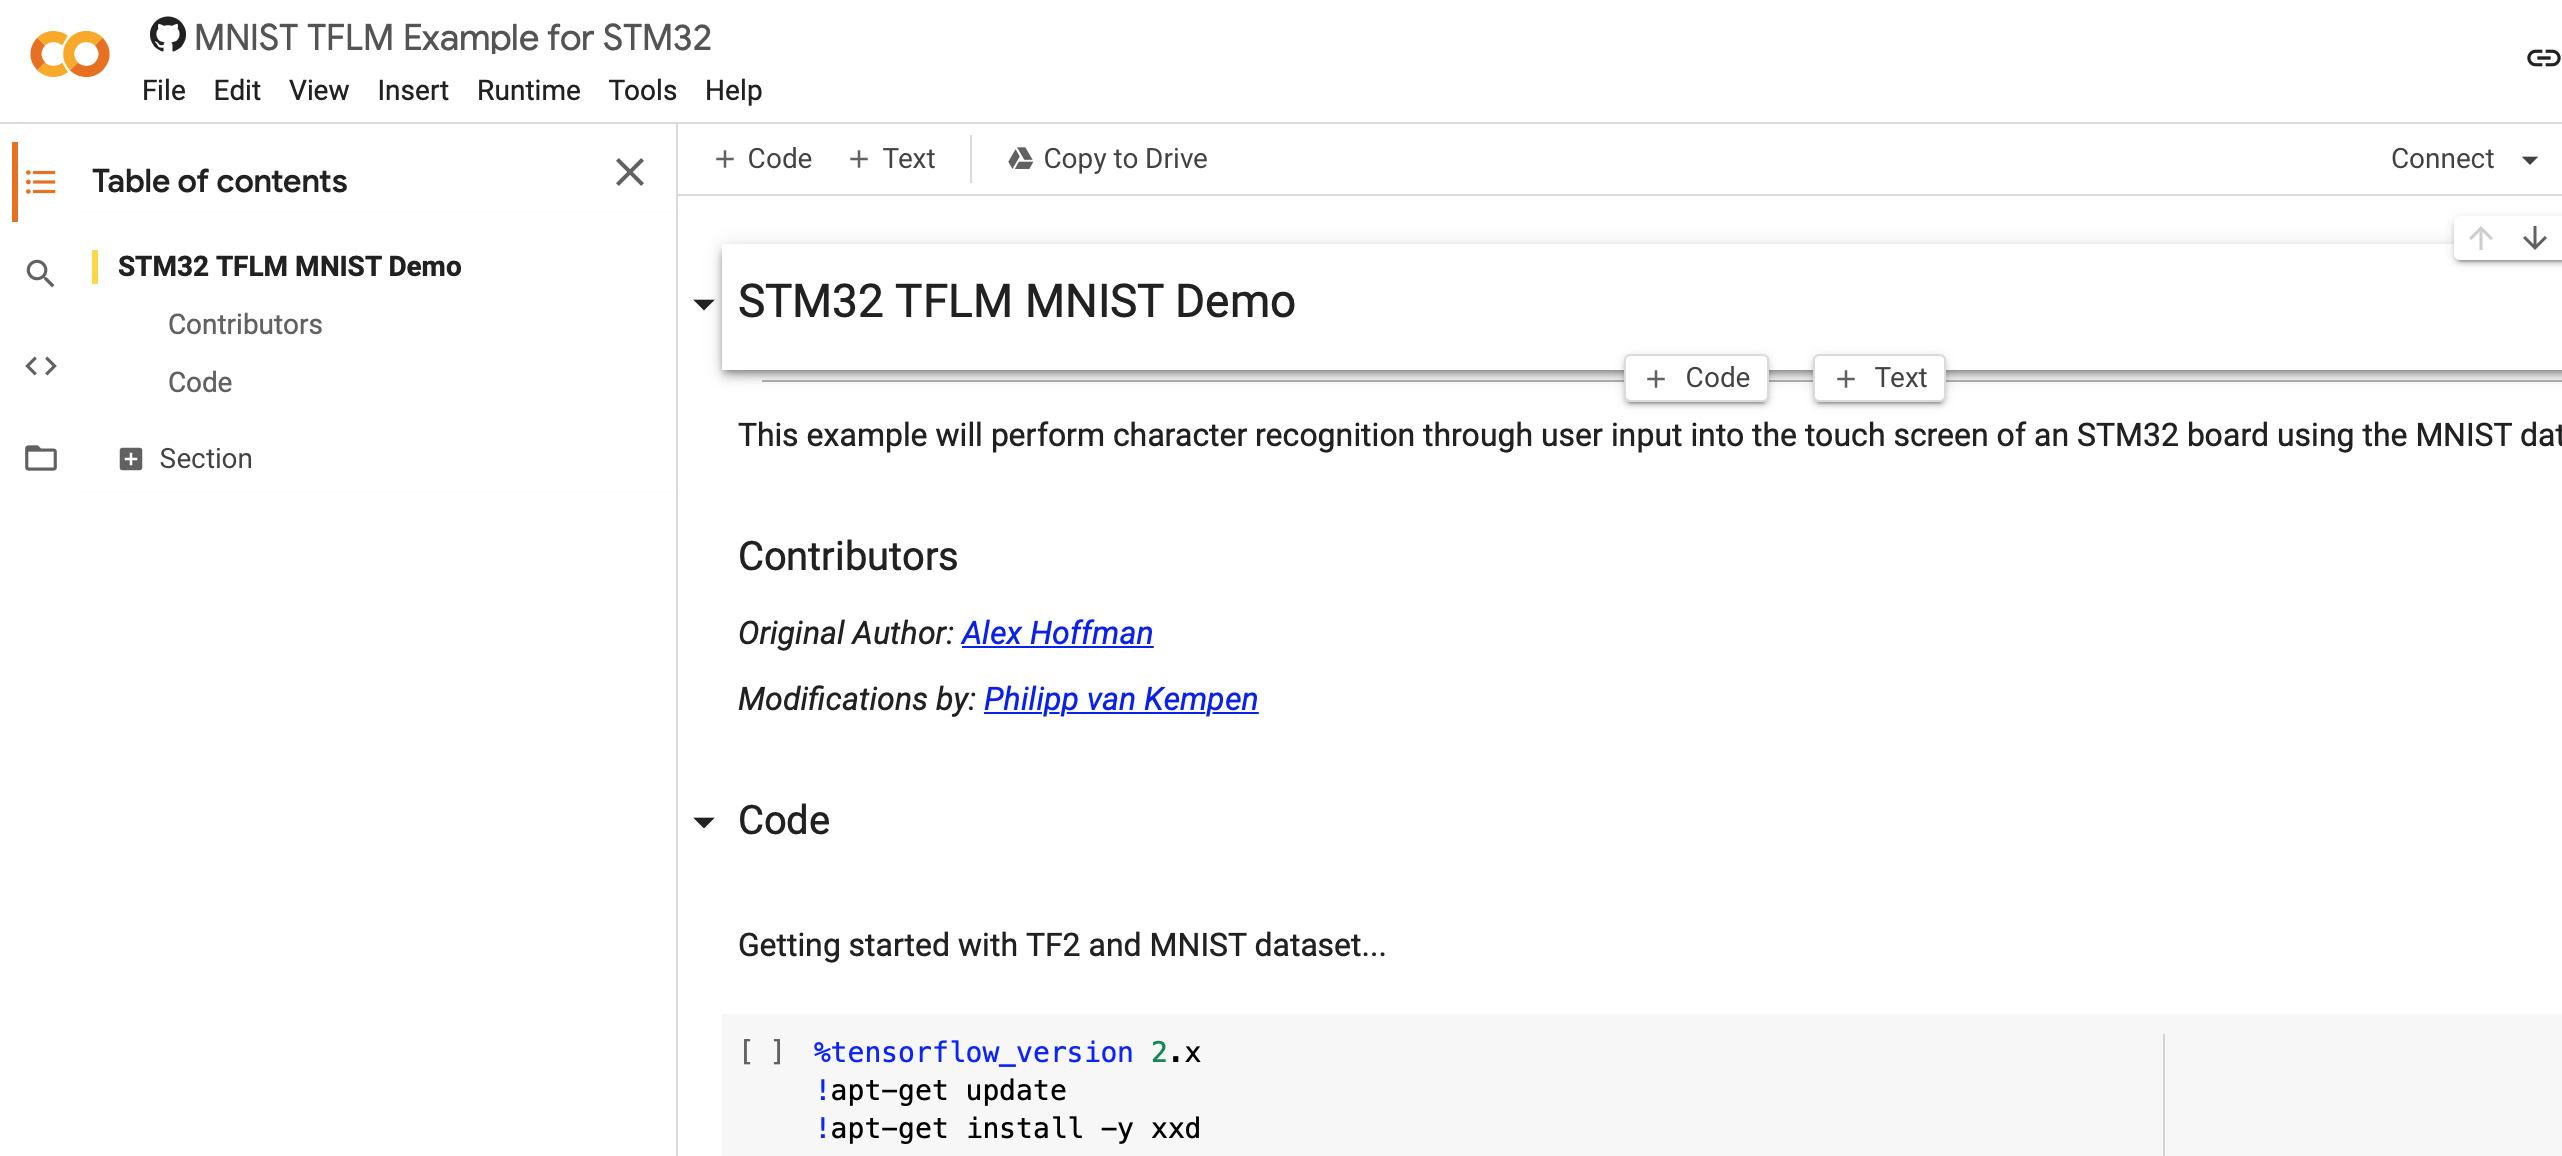
\includegraphics[width=.7\textwidth]{figures/screen_colab.png}
\end{frame}

\begin{frame}

\vspace{-2em}
\begin{figure}[h]
     \centering
     \begin{subfigure}[b]{0.3\textwidth}
         \centering
         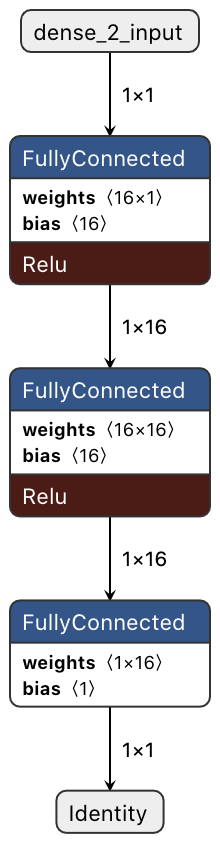
\includegraphics[width=0.3\textwidth]{figures/hello_world_graph.png}
         \caption{Hello World}
         \label{fig:netron_hello_world}
     \end{subfigure}
     \hfill
     \begin{subfigure}[b]{0.3\textwidth}
         \centering
         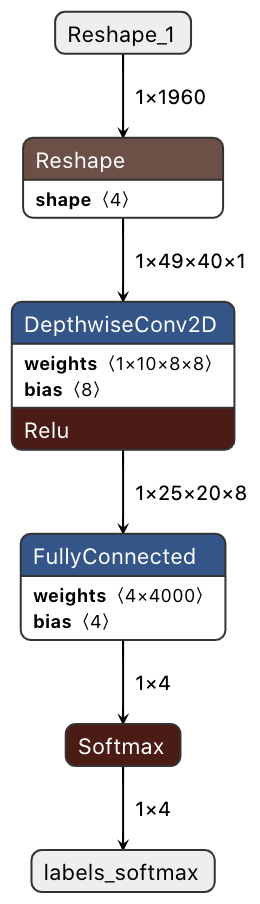
\includegraphics[width=0.4\textwidth]{figures/micro_speech_graph.png}
         \caption{Micro Speech}
         \label{fig:netron_mirco_speech}
     \end{subfigure}
     \hfill
     \begin{subfigure}[b]{0.3\textwidth}
         \centering
         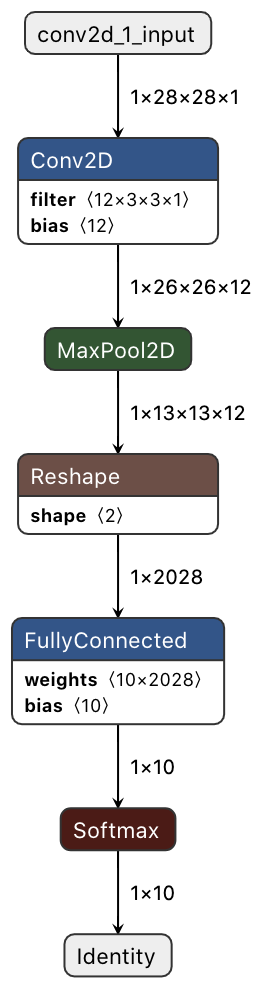
\includegraphics[width=0.4\textwidth]{figures/mnist_graph.png}
         \caption{MNIST}
         \label{fig:netron_mnist}
     \end{subfigure}
        \caption{TFLite Model Graphs per Example}
        \label{fig:netron}
\end{figure}

\end{frame}

\begin{frame}
  \frametitle{Implementation}

\begin{itemize}
    \item \textbf{Hello World:} Ran almost out of the box
    \item \textbf{Micro Speech:}
    \begin{itemize}
        \item Hardest challenge: Streaming real-time audio
        \item Boards to slow? $\Rightarrow$ Solution: Enable CMSIS-NN
        \item Further Tuning of parameters was required to detect any voice commands $\Rightarrow$ More false positives!
    \end{itemize}
    \item \textbf{MNIST:}
    \begin{itemize}
        \item Dataset: ten-thousands of handwritten digits
        \item Quantization issue: Latest TFLM does not support unsigned uint8 inputs $\Rightarrow$ transform to $\{-128,\ldots,127\}$
        \item Challenge: Transform touchscreen input into 28x28 pixel grayscale images
        \item Bug in Alex's implementation: Inverted colors
        \item Some digits can not be detected at all $\Rightarrow$ Improve network architecture
    \end{itemize}
    \item Common:
    \begin{itemize}
        \item Added Benchmarking module
        \item Added Memory Reporting support
        \item Added possibility to choose TFLM interpreter or compiler
        \item For easier Testing: SD-Card support to feed real samples to the network
    \end{itemize}
\end{itemize}
\end{frame}

\begin{frame}
\begin{figure}[h]
     \centering
     \begin{subfigure}[b]{0.3\textwidth}
         \centering
         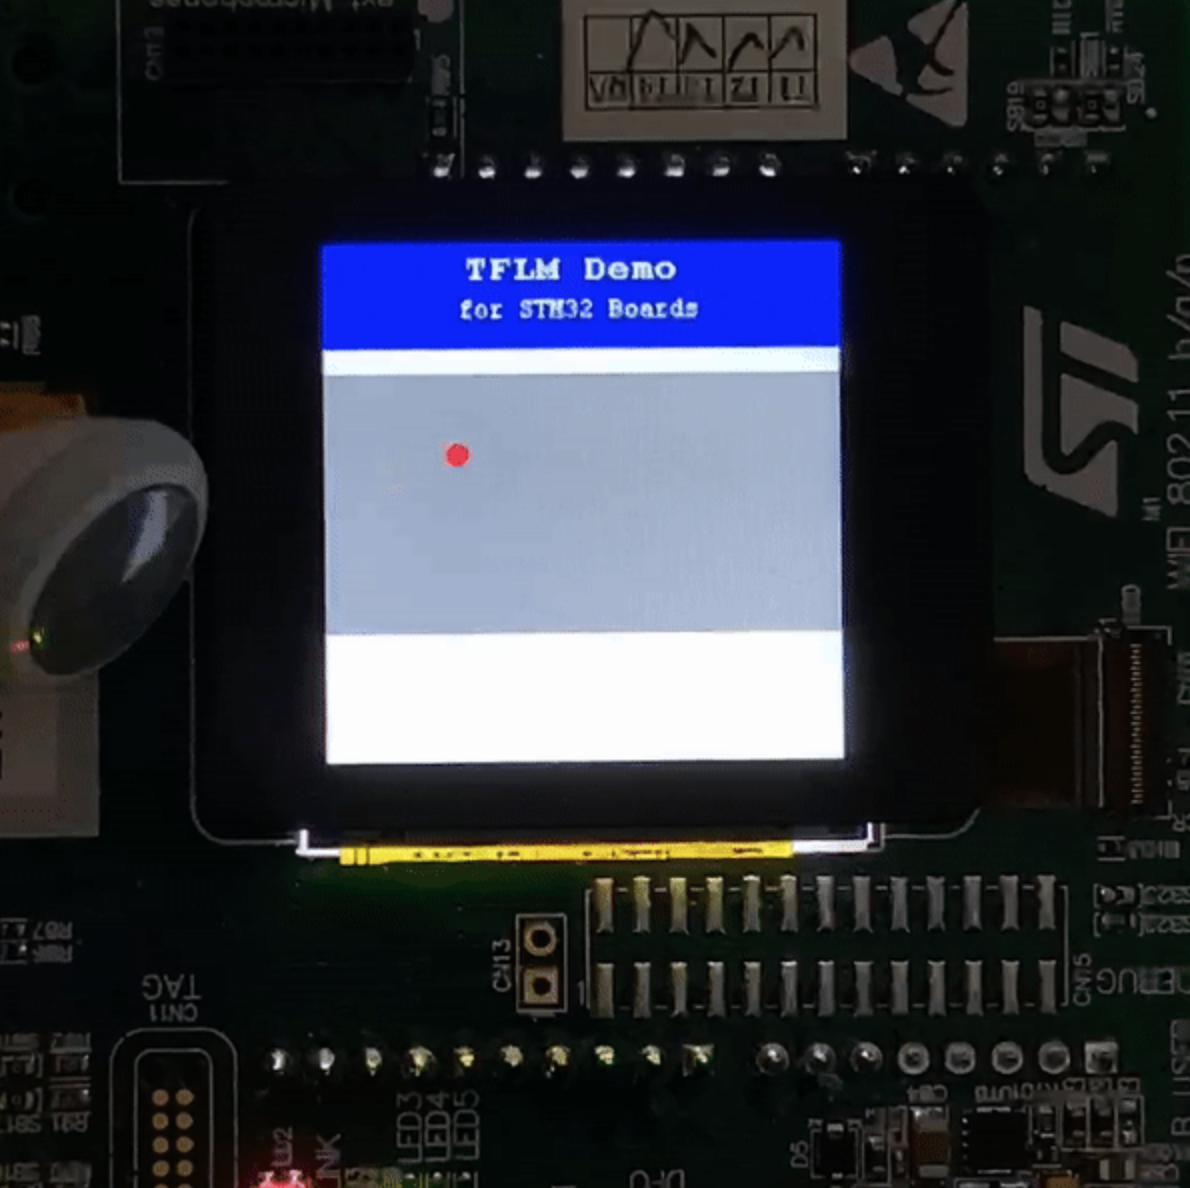
\includegraphics[width=0.8\textwidth]{figures/hello_world_gif.png}
         \caption{Hello World}
         \label{fig:gif_hello_world}
     \end{subfigure}
     \hfill
     \begin{subfigure}[b]{0.3\textwidth}
         \centering
         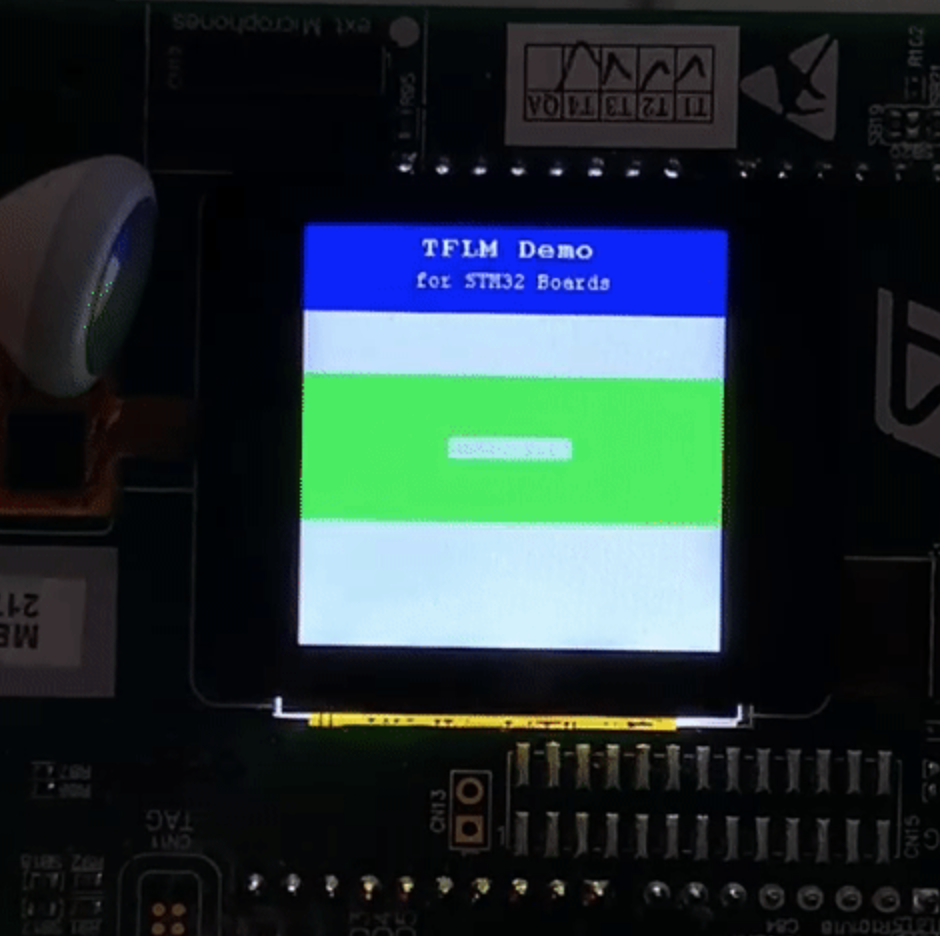
\includegraphics[width=0.8\textwidth]{figures/micro_speech_gif.png}
         \caption{Micro Speech}
         \label{fig:gif_mirco_speech}
     \end{subfigure}
     \hfill
     \begin{subfigure}[b]{0.3\textwidth}
         \centering
         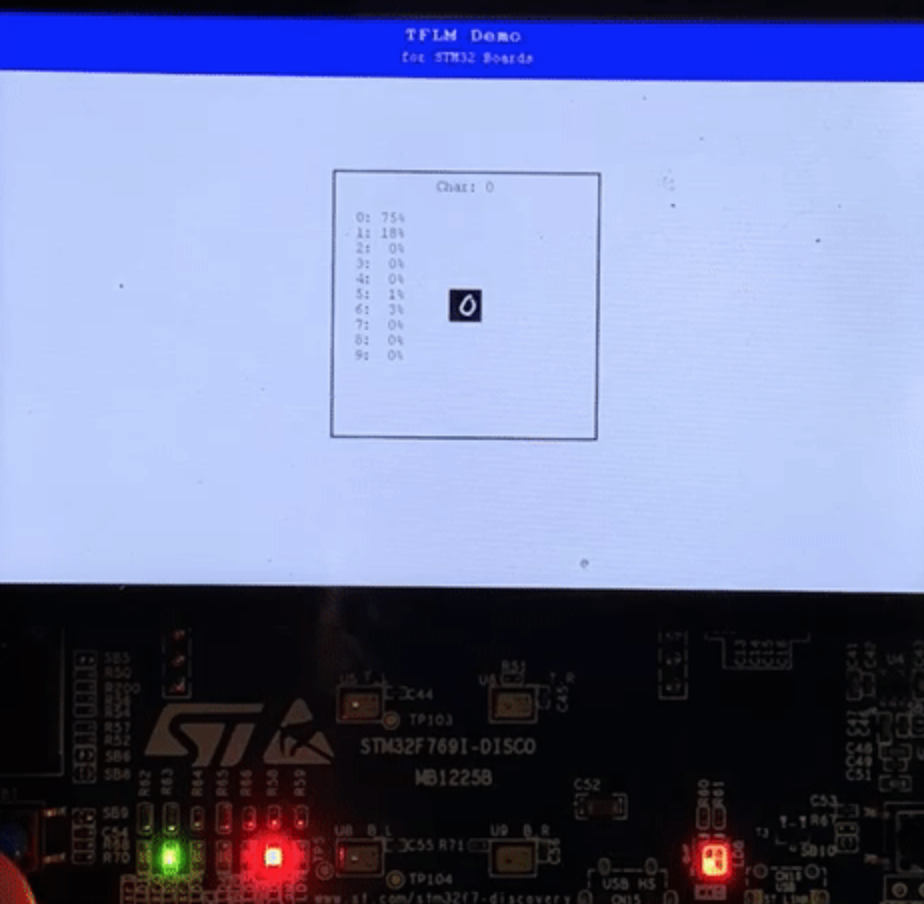
\includegraphics[width=0.8\textwidth]{figures/mnist_gif.png}
         \caption{MNIST}
         \label{fig:gif_mnist}
     \end{subfigure}
        \caption{Examples running on the STM32 Boards\footnote{See \url{https://github.com/PhilippvK/stm32-tflm-demos} for GIFs!}}
        \label{fig:gifs}
\end{figure}

\end{frame}

\begin{frame}
  \frametitle{Documentation}
  
  \centering{
  \begin{itemize}
      \item Common toolchain parts as submodules $\Rightarrow$ less redundant code
      \item Wrapper repository\footnote{\url{https://github.com/PhilippvK/stm32-tflm-demos}}
      \item Common documentation at a single place
      \item Great Extend-ability
  \end{itemize}}
  
  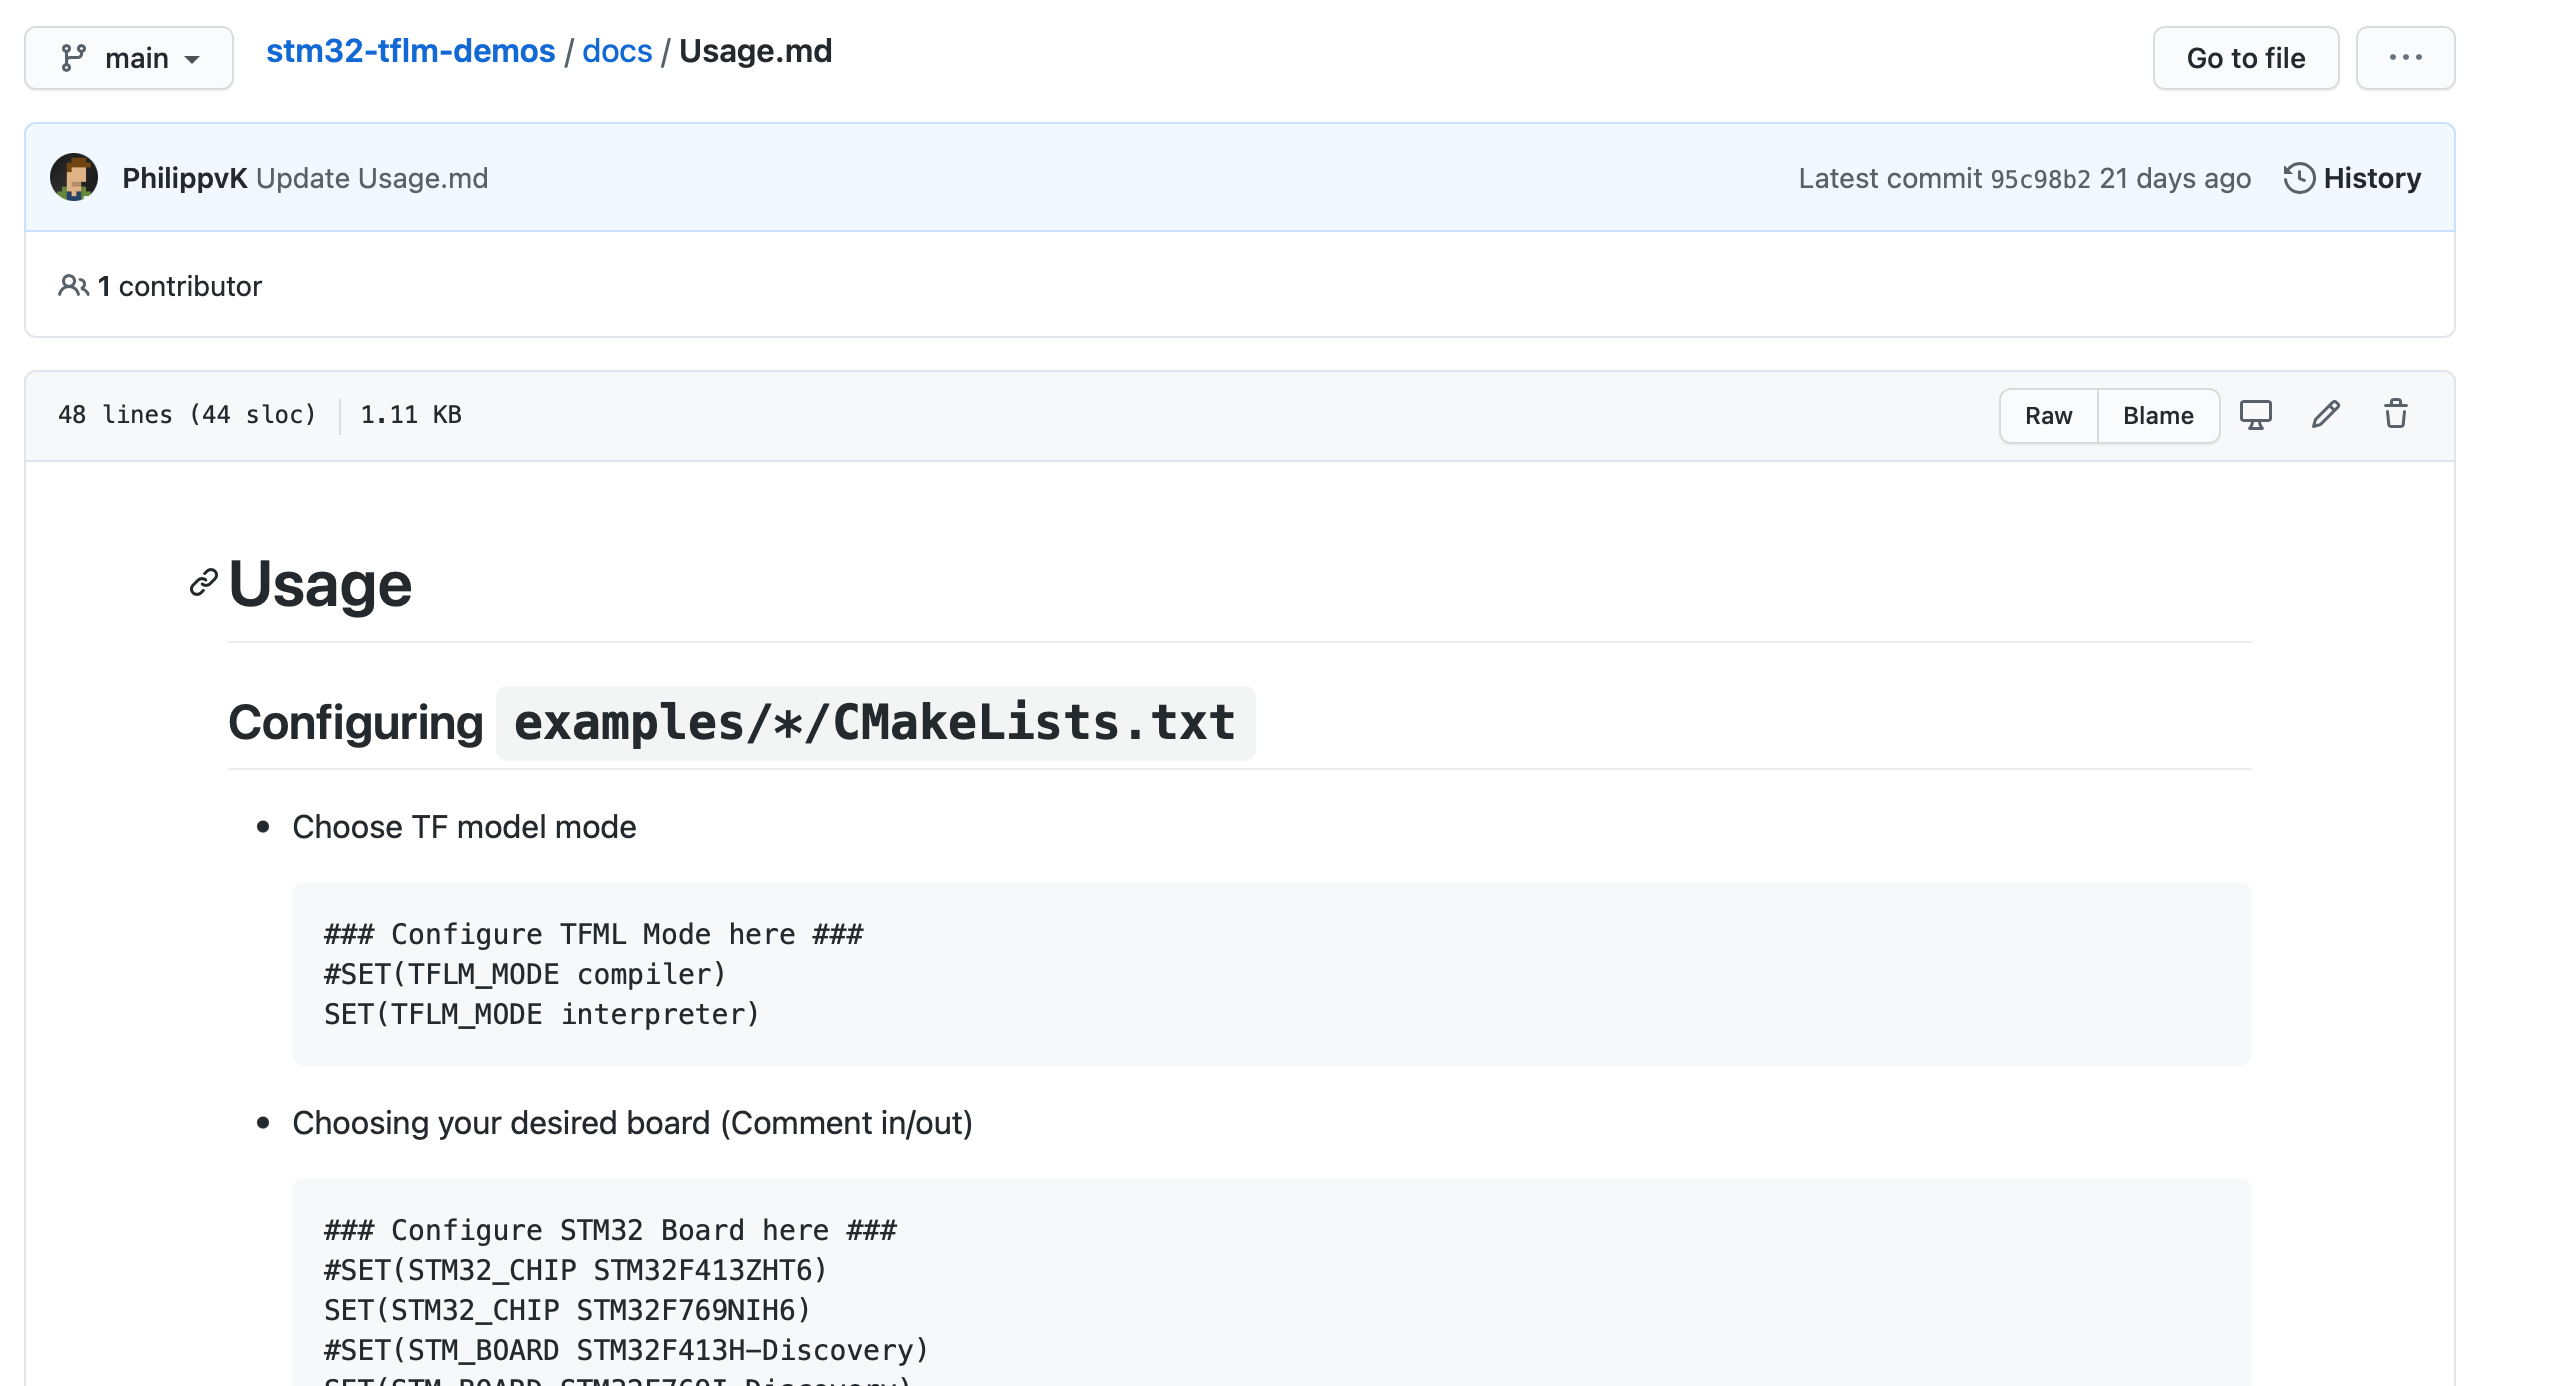
\includegraphics[width=.5\textwidth]{figures/docs.png}

\end{frame}

\begin{frame}
  \frametitle{Evaluation}
  See report PDF or Documentation\footnote{\url{https://github.com/PhilippvK/stm32-tflm-demos/blob/main/docs/Metrics.md}} for details! Only showing tables here...
\begin{figure}[h]
     \centering
  \begin{table}[h]
\begin{tabular}{|l|c|c|l|}
\hline
& \multicolumn{2}{c|}{\textbf{Boards}} &\\\hline
\textbf{Metrics} & STM32F413HDISCOVERY & STM32F769IDISCOVERY & \textbf{Units} \\\hline
Clock Frequency   & 100  & 216    & \textit{MHz}         \\
Special Features  & -        & Double Issue, I/D-Cache      & \textit{-}       \\
Flash Memory      & 1.5      & 2      & \textit{MB}          \\
SRAM Memory       & 256                              & 512                              & \textit{kB}    \\\hline
\end{tabular}
\end{table}
 \caption{Board Metrics}
\end{figure}

\end{frame}

\begin{frame}
  \frametitle{Evaluation - Memory Usage \& Number of Ops}

\begin{figure}[h]
     \centering
  \begin{table}[h]
\begin{tabular}{|l|c|c|c|l|}
\hline
& \multicolumn{3}{c|}{\textbf{Examples}} &\\\hline
\textbf{Type}                        & hello\_world & mirco\_speech & mnist & \textbf{Units} \\\hline
Model Size (FLASH)                      & 2              & 18              & 23      & \textit{kB}     \\
TensorArena Size (SRAM) & 1              & 7               & 11      & \textit{kB}\\\hline  
\end{tabular}
\end{table}
 \caption{Memory Usage (approx.)}
\end{figure}

\begin{figure}[h]
     \centering
\begin{table}[h]
\begin{tabular}{|c|c|c|}
\hline
\multicolumn{3}{|c|}{\textbf{Examples}}\\\hline
hello\_world & mirco\_speech & mnist        \\\hline
41 \textit{FLOPS}     & 689980 \textit{FLOPS}  & 202810 \textit{FLOPS}\\\hline
\end{tabular}
\end{table}
 \caption{Number of Ops (after quant.)}
\end{figure}

\end{frame}

\begin{frame}
  \frametitle{Evaluation - Runtime Measurements \& CMSIS-NN}

\begin{figure}[h]
     \centering
\begin{table}[h!]
\begin{tabular}{|l|l|c|c|c|l|}
\hline
& &\multicolumn{3}{c|}{\textbf{Examples}} &\\\hline
\textbf{Section} & \textbf{CPU} & hello\_world  & mirco\_speech & mnist                                         & \textbf{Units} \\\hline
\multirow{2}{*}{Populate}     &  F4              & $\sim$0 & 38 & 132 & \multirow{2}{*}{\textit{ms}} \\
&F7&$\sim$0&11&88&\\\hline
\multirow{2}{*}{Invoke}     &  F4              & $\sim$0 & 49 & 34 & \multirow{2}{*}{\textit{ms}} \\
&F7&$\sim$0&52&13&\\\hline
\multirow{2}{*}{Respond}     &  F4              & $\sim$0 & $\sim$0 & 125 & \multirow{2}{*}{\textit{ms}} \\
&F7&$\sim$0&$\sim$0&93&\\\hline
\end{tabular}
\end{table}
 \caption{Runtime Measurements (approx.)}
\end{figure}

\begin{figure}[h]
     \centering
\begin{table}[h]
\begin{tabular}{|l|l|l|l|l|l|}
\hline
\multicolumn{2}{|l|}{} & \multicolumn{3}{c|}{\textbf{Examples}} &\\\hline
\multicolumn{2}{|l|}{\textbf{Settings}}  & hello\_world & mirco\_speech & mnist & \textbf{Units} \\\hline
\multirow{2}{*}{CMSIS\_NN} & OFF              & $\sim$1                 & 413 (unusable!)                 & 52               & \textit{ms}             \\
 & ON               & $\sim$0                 & 52                       & 13               & \textit{ms}              \\\hline
\multicolumn{2}{|l|}{Difference}                   & (?)                     & (-87)                    & (-75)            & \textit{\%}           \\\hline  
\end{tabular}
\end{table}
 \caption{CMSIS-NN Improvements (approx.)}
\end{figure}
  %\footfullcite{jirauschek2014}

\end{frame}

\begin{frame}
  \frametitle{Conclusions and Outlook}

  \begin{itemize}
  \item Main goal fulfilled
  \item MNIST was optional but also implemented successfully
  \item Models need more tuning
  \item Demonstrated capabilities of TinyML on microcontroller platforms
  \end{itemize}

  \pause

  \textbf{Future Work:}

\begin{itemize}
    \item Support USB-Storage as alternative to SD-Card
    \item Add TinyFace Model\footnote{\url{https://github.com/munober/thesis/blob/master/digital_edition.pdf}}
    \item Merge Deployment and Evaluation Flow with EDA RISCV-toolchain
    \item Enable usage of FreeRTOS instead of baremetal
    \item Add possibility to parse results via UART
    \item Feed samples via UART for automated testing\\[1em]
    $\Rightarrow$ Extract data on the accuracy of the models
\end{itemize}



\end{frame}

\end{document}
